\chapter{Server-Side Implementation}
\lhead{\emph{Server-Side Implementation}}
\label{chapter:server}

The purpose of the server is to receive image data from the rover, produce a 3D environment from this data, and feed back control inputs from the user. This is all done within the framework of the 3D game engine Unreal Engine 4 \cite{unreal}. Unreal 4 was chosen because it supports almost any VR headset on the market, is simple to integrate with OpenCV, and is free to use. The structure of any Unreal program is very complicated, as the engine does a lot in the background across many threads. The implementation of this project within the Unreal environment (Figure \ref{fig:unreal}) consists of a receive thread that receives images, processes them, then updates the 3D model, and a portion of the game thread (the Unreal thread that handles game logic) that handles and sends user input 20 times a second. The fact that the 3D model is updated on a thread separate to the rendering of the images that are sent to the headset is what allows the headset to run at an unrelated and significantly faster frame rate than the model is being updated at.

\begin{figure}[H]
    \begin{center}
      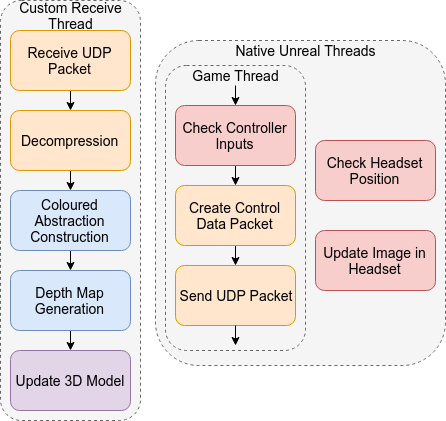
\includegraphics[width=0.75\textwidth]{Figures/Unreal.png}
      \caption[Server Program Structure]{Server Program Structure. Red blocks are standard Unreal functionality, yellow blocks are communications related, blue blocks are OpenCV based, and the purple block is custom integration with the Unreal environment. The blocks within the game thread run 20 times a second. When these blocks are not running, the game thread is handling other game logic within the environment.}
      \label{fig:unreal}
    \end{center}
\end{figure}

\section{Depth Map and Abstraction Construction}

For a depth mapping algorithm to function accurately, the 2 images it receives must be rectified (established in Section \ref{subsection:depth}). The rectification parameters for the cameras in our system have been calculated using a set of programs provided by Sourish Ghost \cite{calibgit}. The rectification is applied using these parameters just before the depth maps are calculated (Figure \ref{fig:rect}).

\begin{figure}[H]
    \begin{center}
    \begin{tabular}{ c c }
        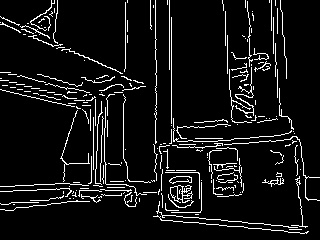
\includegraphics[width=0.45\textwidth]{Figures/prerectL.jpg} &
        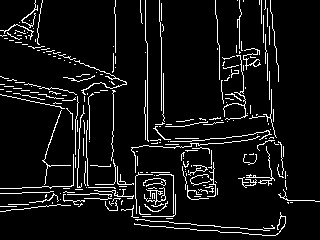
\includegraphics[width=0.45\textwidth]{Figures/prerectR.jpg} \\
        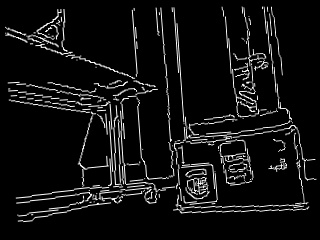
\includegraphics[width=0.45\textwidth]{Figures/postrectL.jpg} &
        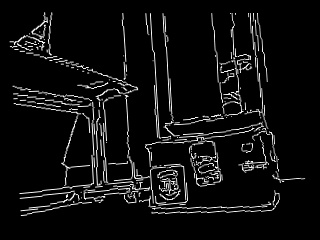
\includegraphics[width=0.45\textwidth]{Figures/postrectR.jpg}
    \end{tabular}
    \caption[Demonstration of Stereo Image Rectification]{Demonstration of Stereo Image Rectification. The original left and right images are shown top left and top right, with their rectified counterparts bottom left and bottom right. It can be seen that the features of the bottom images are better matched vertically than in the original images.}
    \label{fig:rect}
    \end{center}
\end{figure}

When selecting a depth mapping algorithm, the major factors to consider were speed and performance with abstracted images. The use of abstractions makes demonstrations of the algorithms with normal images of little help; there is no guarantee that the algorithms would be able to map depth for edge detected lines with the same accuracy, if at all, since this is not what they were designed for. Three different depth mapping algorithms were tested: StereoBM, StereoSGBM, and Libelas. StereoBM and StereoSGBM are a block matching and semi block matching algorithm provided by OpenCV \cite{OpenCV}, and Libelas is a more complex algorithm provided by the Autonomous Vision Group \cite{geiger2010efficient}. Of the three algorithms presented, StereoBM is the fastest and Libelas the slowest (Figure \ref{fig:speed}). 

\begin{figure}[H]
    \begin{center}
      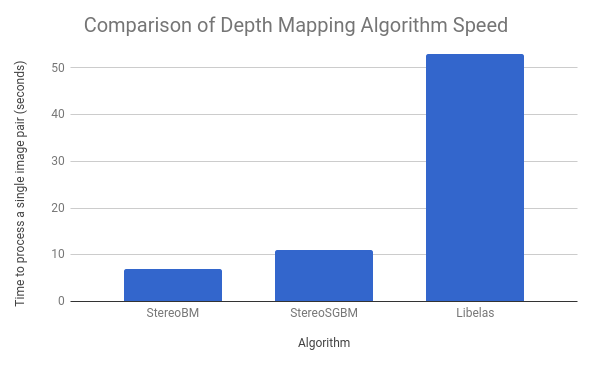
\includegraphics[width=0.8\textwidth]{Figures/depthspeed.png}
      \caption[Comparison of Depth Mapping Algorithm Speed]{Comparison of Depth Mapping Algorithm Speed. The test images used to produce this data were the rectified images presented in Figure \ref{fig:rect}. These same images were used in the production of all further figures in this section.}
      \label{fig:speed}
    \end{center}
\end{figure}

When tested on images received from the rover, StereoBM and StereoSGBM produced noisy results, yet, if inspected closely, results that include reasonable depth information along the areas where edges were in the original images (Figure \ref{fig:MappingComp}). Libelas, however, did not produce results that were in any way recognisable. Combining this with its significantly slower processing speed, it is clear that Libelas is not that correct choice for this use case.

\begin{figure}[H]
    \begin{center}
    \begin{tabular}{ c c }
        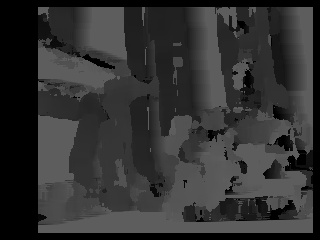
\includegraphics[width=0.45\textwidth]{Figures/BMout.jpg} &
        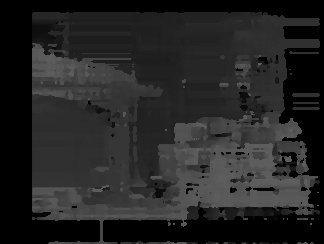
\includegraphics[width=0.45\textwidth]{Figures/sgbmout.jpg} \\
        \multicolumn{2}{c}{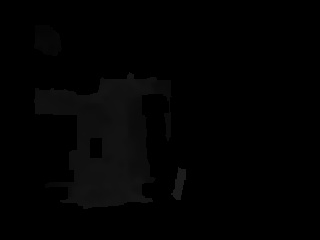
\includegraphics[width=0.45\textwidth]{Figures/libelasout.jpg}}
    \end{tabular}
    \caption[Comparison of Raw Depth Mapping Algorithm Output]{Comparison of Raw Depth Mapping Algorithm Output. The StereoBM output (top left) is very noisy, however correct depth can be seen on the box in the bottom right and on the table in the top left (when compared to the input images in Figure \ref{fig:rect}). The StereoSGBM output (top right) shows similar results, though with a significant reduction in noise. The Libelas output (bottom) shows very little- it does not seem to work with edge detected images whatsoever.}
    \label{fig:MappingComp}
    \end{center}
\end{figure}

To be able to compare StereoBM and StereoSGBM further, the noise their outputs contain must be filtered out. This can be achieved by applying Weighted Least Squares filtering to the depth map (Figure \ref{fig:filtered}). This is effective in producing consistent depth across the objects in the map. Unfortunately, regardless of the angle to the camera that an object sits at, the filtering will often assign it a single depth across the whole surface. This results in surfaces like the floor or the ceiling being inaccurately represented as a vertical plane very close to the camera, however most other objects are not significantly affected.


\begin{figure}[H]
    \begin{center}
      \begin{tabular}{ c c }
        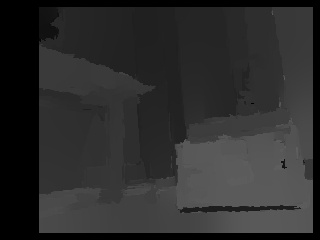
\includegraphics[width=0.45\textwidth]{Figures/BMfiltered.jpg} &
        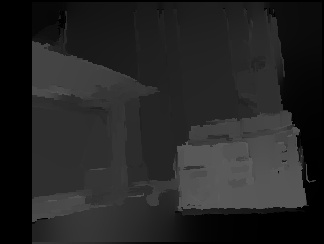
\includegraphics[width=0.45\textwidth]{Figures/sgbmfilt.jpg}
      \end{tabular}
      \caption[Filtered StereoBM and StereoSGBM Outputs]{Filtered StereoBM and StereoSGBM Outputs. The StereoBM output (left) has been improved significantly by the filtering, with mostly consistent and correct depth across all objects other than the floor. StereoSGBM (right) has been similarly cleaned up, however has not provided depth for the floor or right wall whatsoever. The single section of floor it attempted (under the table in the bottom left) is the same incorrect depth as produced by StereoBM.}
      \label{fig:filtered}
    \end{center}
\end{figure}

When comparing the filtered maps, there are very few differences. Both are reasonable representations of the original scene, and when one makes a mistake in the depth of an object, the other will probably make the exact same mistake. The only major difference is that StereoBM will consider the floor incorrectly as a vertical plane close to the camera, whereas StereoSGBM will incorrectly not record a depth for it at all. This lack of a significant gain in quality when using the noticeably slower StereoSGBM led to StereoBM being chosen as the algorithm used in the final system.

While the individual depth maps (post filtering) are reasonable approximations of the space being viewed, the depth of a single object with be inconsistent between frames, due to inconsistencies between the edge detected frames they were produced from. When viewed as a video feed, most objects will oscillate slightly, with greater oscillations in objects that are more ambiguous or less consistent in the edge detected frames. This issue is mitigated in the system by taking a running average, the weighting of the frames in the average reducing with the age of the frame. This increases consistency substantially at the expense of a minor reduction in responsiveness.

The construction of the coloured abstraction is as addressed in Chapter \ref{chapter:abstract}. The seed point/average colour pairs are each used to flood fill "Edge Detected Img 1" from Figure \ref{fig:system}, producing the full abstraction that is to be applied as a texture to the 3D model generated from the depth maps.

\section{3D Model Generation}

To generate a 3D model dynamically based on image data, an Unreal Engine 4 class that allows for mesh generation at run-time is required. Although more intelligent options are available as add-ons, the core Unreal 4 class "procedural mesh" was selected due to its simplicity and compatibility with OpenCV. The class is used as a basis for the generation of a grid based mesh (Figure \ref{fig:mesh}).

\begin{figure}[H]
    \begin{center}
      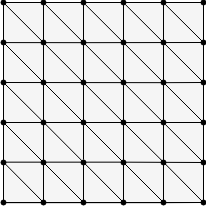
\includegraphics[width=0.6\textwidth]{Figures/mesh.png}
      \caption[Mesh Grid Segment]{Mesh Grid Segment. Each corner of the grid is a vertex, with triangles formed from the vertices. The grid is built in the X-Y plane, leaving the Z component of each vertex available to be easily assigned depth.}
      \label{fig:mesh}
    \end{center}
\end{figure}

Each pixel in the depth map is mapped to a vertex in the mesh, resulting in a grid of 320x240 vertices for 320x240 pixel images. The colour value of each depth map pixel is mapped to the Z component of its corresponding vertex, leading to the bright pixels in the depth map (close objects) generating vertices that are pushed forward from the grid. When this grid is placed an appropriately realistic distance from the the user in the headset, the close objects in the depth map will be pushed closer to the user and the further objects will remain closer to the grid, further from the user. When the full coloured abstraction is then applied to the mesh as a texture, the pixels once again mapping 1:1 to the vertices, the space the rover is observing is finally being portrayed in VR (Figure \ref{fig:3DModel}).

\begin{figure}[H]
    \begin{center}
      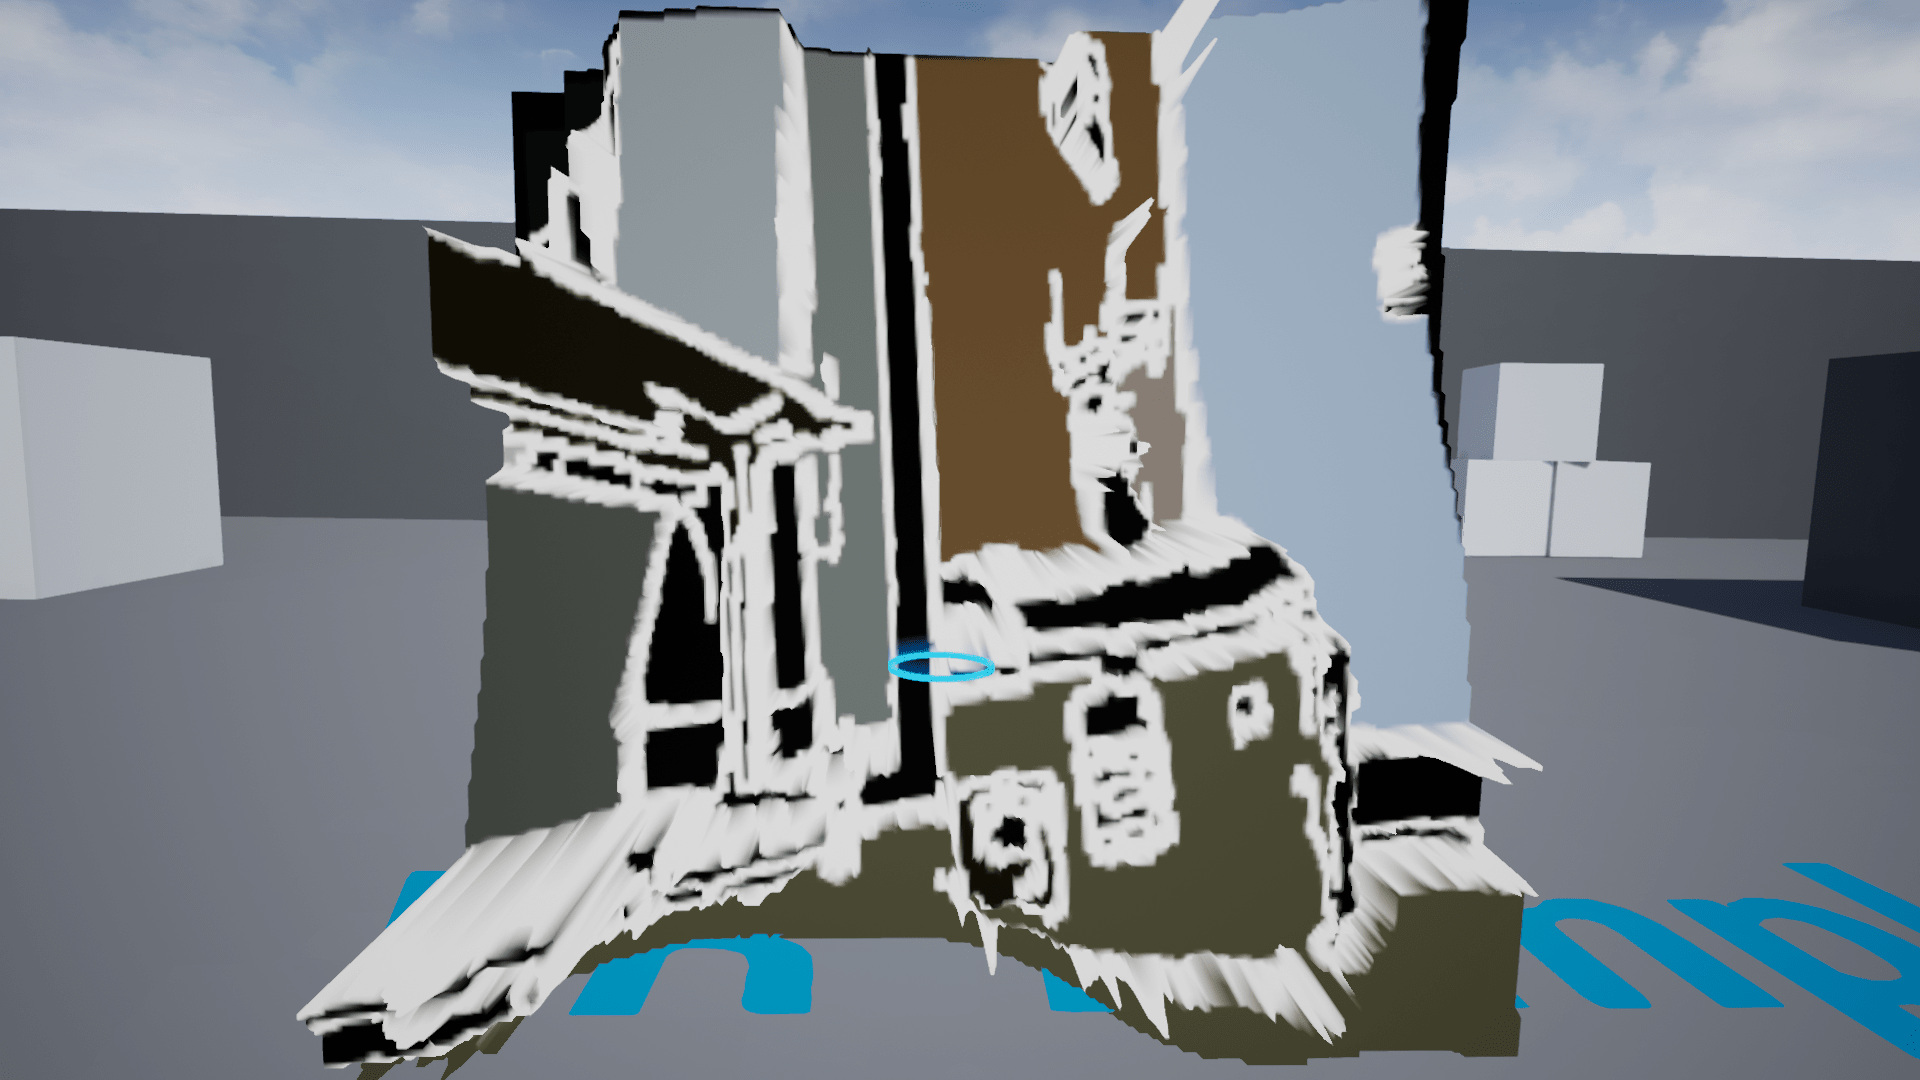
\includegraphics[width=0.9\textwidth]{Figures/OutlinePic2.png}
      \caption[Final Textured 3D Model]{Final Textured 3D Model.}
      \label{fig:3DModel}
    \end{center}
\end{figure}